\chapter{Implementierung}
\label{chap:implementierung}
\todo{Intro zur Implementierung schreiben.}
In der folgenden Übersicht sind die Routen dargestellt, die im Dashboard verfügbar sind. Angegeben wird auch, welche Daten verwendet werden, um die Seite dynamisch mit Inhalt zu füllen.

\begin{itemize}
    \item \textbf{/ (Startseite):} Statische Startseite des Dashboards mit Buttons zur Navigation zu anderen Routen.
    
    \item \textbf{/mitre/kubernetes\_matrix (Kubernetes Matrix):} Visualisierung der angepassten \gls{mitre} \gls{attack} Matrix.
    \begin{itemize}
        \item \textbf{Dynamisch erzeugt aus:}
        \begin{itemize}
            \item \textbf{kubernetes\_matrix.tmpl:} Nutzt die Anzahl der Taktiken und Techniken zum Aufbau der Zeilen und Spalten. 
            \item \textbf{technique.partial.tmpl:} Füllt die Felder mit den in \verb|pkg/mitre/technique.go| definierten Techniken.
        \end{itemize}
    \end{itemize}
    
    \item \textbf{/artifacts (Artefakte - Index):} Liefert eine Liste aller Artefakte, aller Filtermöglichkeiten und einer visuellen Darstellung auf der Zeitachse.
    \begin{itemize}
        \item \textbf{Query-Parameter (optional):}
        \begin{itemize}
            \item \texttt{tool\_name} - Filtert Artefakte nach dem Namen des Tools.
            \item \texttt{tactic} - Filtert Artefakte nach der zugehörigen Taktik.
            \item \texttt{microsoft\_technique} - Filtert Artefakte nach Microsoft-Techniken.
            \item \texttt{start\_date} - Filtert Artefakte nach Startzeitpunk.
            \item \texttt{end\_date} - Filtert Artefakte nach Endzeitpunkt.
        \end{itemize}
        \item \textbf{Dynamisch erzeugt aus:} 
        \begin{itemize}
            \item \textbf{artifacts/index.tmpl:} Nutzt die Daten aller Artefakte und die Werte der Filterparameter.
        \end{itemize}
    \end{itemize}
    
    \item \textbf{/artifacts/:id (Artefakte - Details):} Liefert Details zu einem spezifischen Artefakt anhand der \texttt{id}.
    \begin{itemize}
        \item \textbf{Dynamisch erzeugt aus:} 
        \begin{itemize}
            \item \textbf{artifacts/show.tmpl:} Nutzt die Daten eines Artefaktes.
            \item \textbf{error.tmpl:} Spezifische Fehlermeldung von \textit{Go} nach Datenbankabfrage.
        \end{itemize}

    \end{itemize}
    
    \item \textbf{/campaigns (Kampagnen - Index):} Liefert eine Liste aller Kampagnen.
    \begin{itemize}
        \item \textbf{Dynamisch erzeugt aus:}
        \begin{itemize}
            \item \textbf{campaigns/index.tmpl:} Nutzt die Daten aller Artefakte und die Werte der Filterparameter.
        \end{itemize}
    \end{itemize}
    
    \item \textbf{/campaigns/:id (Kampagnen - Details):} Liefert Details zu einer spezifischen Kampagne anhand der \texttt{id}.
    \item \textbf{Query-Parameter (optional):}
        \begin{itemize}
            \item \texttt{start\_date} - Filtert Kampagnen nach Startzeitpunk.
            \item \texttt{end\_date} - Filtert Kampagnen nach Endzeitpunkt.
        \end{itemize}
    \begin{itemize}
        \item \textbf{Dynamisch erzeugt aus:}
        \begin{itemize}
            \item \textbf{campaigns/show.tmpl:} Nutzt die Daten einer Kampagne.
            \item \textbf{error.tmpl:} Spezifische Fehlermeldung von \textit{Go} nach Datenbankabfrage.
        \end{itemize}
    \end{itemize}
\end{itemize}

\section[Anwendung von ACEMA]{Anwendung von ACEMA auf das Dashboard}
\label{sec:impl-anwendungVonAcema}
\todo{Dieses Kapitel benötigt noch viel Arbeit.}
\todo{Hier muss erstmal noch erklärt werden, wie aus den in Go Code definierten Techniken der Input für ACEMA generiert wird.}

Die Funktionen, die die Datenverarbeitung aus der \verb|json| Datei vornehmen, arbeiten nicht direkt mit dem Output von \gls{acema} (Dateiname: \verb|t-cwe-cve-dict.json|), sondern mit einer eigens leicht abgewandelten Version, in der nur die für das Dashboard relevanten Daten vorhanden sind. Der abgewandelten Quellcodes sind im Fork \autocite{jesseDumpeldownAcema_oranDev} des Repositories \autocite{klement2023acema} \todo{Und im Anhang?? Das sind aber circa 800 Zeilen Code.} verfügbar. Diese \textit{neue} Datei mit dem Suffix \textit{\_small} wird über das Ausführen von \verb|data_analysis_nb.py| erstellt. Darin sind nur die Daten enthalten, die für die Integration einer Bewertung nach \gls{cvss} nötig sind. Anstatt 43 Zeilen beanspruchen die Daten über einen CVE nur noch sechs Zeilen und beschränken sich auf \gls{cve}-ID, und vier Metriken aus zwei Metrikgruppen die in \gls{cvss}\textit{v2} definiert sind \autocite{CVSSV2Complete}. Details über die Inhalte der Metrikgruppen werden in Kapitel \ref{sec:impl-cvssIntegration} beschrieben.

Es wurden weitere Anpassungen des verfügbaren \gls{acema}-Quellcodes vorgenommen, die den Entwicklungsfluss vereinfachen und Verbesserungen vornehmen. Die Implementierung lässt sich in zwei Teile spalten: den \verb|Gathering|-Teil (deutsch: Sammlungsteil) und den \verb|Analysis|-Teil (deutsch: Analyseteil). Es existieren hierfür jeweils eine Datei mit den aufrufbaren Funktionen und eine andere, die die Aufrufe dieser Funktionen tätigt und prozedural ausgeführt wird und auch so gelesen werden kann.
Die prozeduralen Teile sind im originalen Repository als \verb|jupyter notebooks| (\verb|.ipynb|-Dateien) geschrieben \autocite{klement2023acema,ProjectJupyter}. Diese Dateien wurden zu einfacheren Ausführung in \verb|.py| Dateien konvertiert, sodass sie direkt über die Python-\gls{cli} aufrufbar sind.
Eine vorgenommene Verbesserung bezieht sich auf die in Kapitel \ref{sec:limitationen} angesprochene Limitation der \gls{acema} Implementierung in Bezug auf die Vollständigkeit des Daten-Mappings. Es wurde bereits gezeigt, dass die im Folgenden beschriebene Verbesserung\footnote{Die \gls{acema}-Implementierung in \autocite{klement2023acema} wird als originaler Quellcode bezeichnet, die Veränderung in \autocite{jesseDumpeldownAcema_oranDev} als verbesserter Quellcode.} zu der Schöpfung einer größeren Datenmenge aus der Quelle \gls{nvd} führt (siehe Abbildung \ref{tab:comparison_with_diff}).

Der originale Quellcode arbeitet beim Mapping von \gls{mitre}-Technik zu \gls{capec} mit einem \verb|pandas dataframe|. \textit{Pandas} ist eine bekannte Datenanalysebibliothek für Python \autocite{PandasPythonData}. Für das Konvertieren von \gls{stix}-Daten zu einem \verb|dataframe| wird die Funktion \verb|stixToDf| des \textit{mitreattack} Modules genutzt \autocite{MitreattackpythonMitreattackAttackToExcel}. Wie bereits in Kapitel \ref{sec:limitationen} beschrieben, wird dadurch nur der \textit{enterprise-attack}-Teil der \gls{cti} Daten genutzt. Viele Beziehungen zwischen \gls{mitre}-Technik und \gls{capec} finden sich jedoch auch im \textit{capec/2.1/attack-pattern} Teil des Repositories. Deshalb nutzt die verbesserte Implementierung die Datensätze aus beiden Teilen. Auch wurde ein anderer Ansatz zur Verarbeitung der einzelnen \verb|json|-Dateien angewandt. Anstatt der Konvertierung zu einem mächtigen \verb|dataframe| der alle Daten enthält, werden die \gls{stix}-Daten aus jeder \verb|json|-Datei einzeln geladen und der Inhalt der \gls{stix}-Objekte über \verb|stix_data.get()| ausgelesen \autocite{OasisopenCtipythonstix2OASIS}. Die genaue Abfolge der abgefragten Kriterien bis zum Finden eines Mappings in Abbildung \ref{fig:detailed-mapping} ist als detaillierte Ansicht des Schrittes 1 in Abbildung \ref{fig:mitre_mapping} zu verstehen.

\usetikzlibrary{shapes.geometric, arrows}

\tikzstyle{startstop} = [rectangle, rounded corners, minimum width=0cm, minimum height=0cm, text centered, draw=black, fill=red!30]
\tikzstyle{process} = [rectangle, minimum width=0cm, minimum height=0cm, text centered, draw=black, fill=blue!30]
\tikzstyle{decision} = [diamond, minimum width=0cm, minimum height=0cm, text centered, draw=black, fill=green!30]
\tikzstyle{arrow} = [thick,->,>=stealth]


\begin{figure}
    \centering
    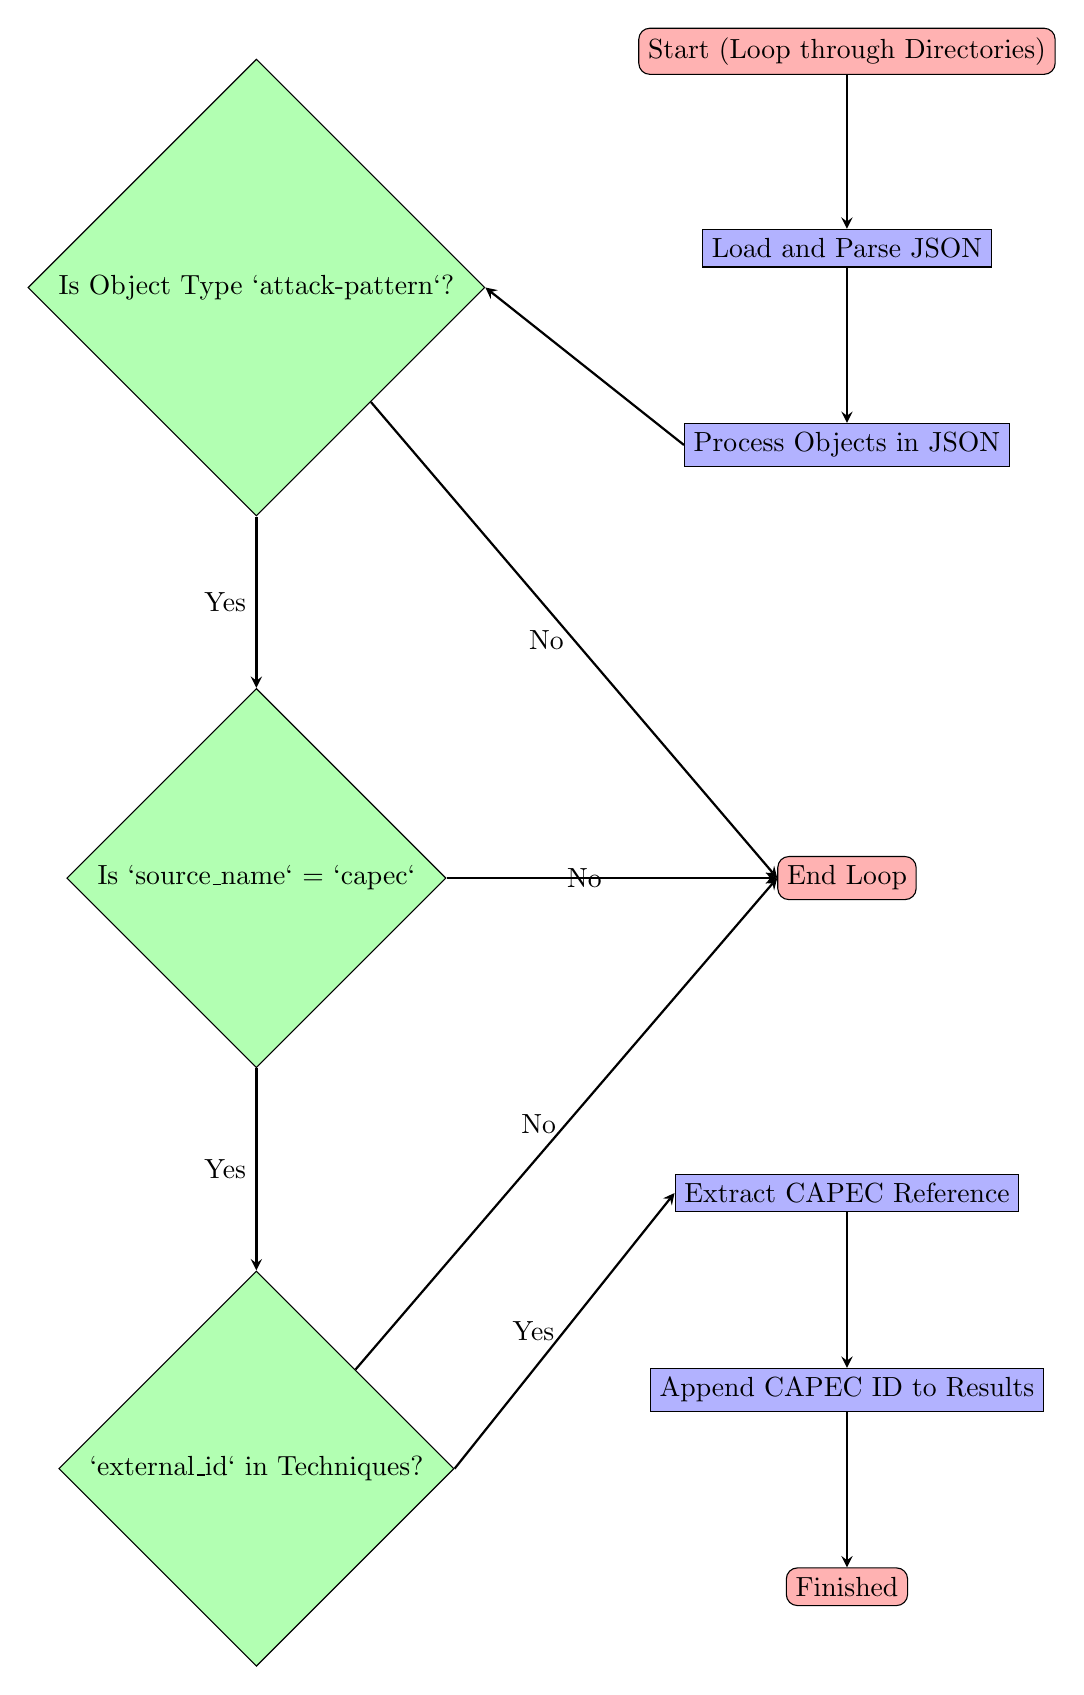
\begin{tikzpicture}[node distance=2.5cm and 3cm]

        % Nodes for processes and start
        \node (start) [startstop] {Start (Loop through Directories)};
        \node (loadJson) [process, below of=start] {Load and Parse JSON};
        \node (processObjects) [process, below of=loadJson] {Process Objects in JSON};
        \node (extractCapec) [process, below of=processObjects, yshift=-7cm] {Extract CAPEC Reference};
        \node (appendCapec) [process, below of=extractCapec] {Append CAPEC ID to Results};

        % Nodes for decisions (aligned left)
        \node (checkType) [decision, left of=start, xshift=-5cm, yshift=-3cm] {Is Object Type `attack-pattern`?};
        \node (checkRef) [decision, below of=checkType, yshift=-5cm] {Is `source\_name` = `capec`};
        \node (checkTechnique) [decision, below of=checkRef, yshift=-5cm] {`external\_id` in Techniques?};

        % Node for Stop and finish
        \node (end) [startstop, right of=checkRef, xshift= +5cm] {End Loop};
        \node (finish) [startstop, below of=appendCapec] {Finished};


        % Arrows from processes to decisions
        \draw [arrow] (processObjects.west) -- (checkType.east);
        \draw [arrow] (start) -- (loadJson);
        \draw [arrow] (loadJson) -- (processObjects);

        % Arrows between decisions
        \draw [arrow] (checkType) -- node[anchor=east] {Yes} (checkRef);
        \draw [arrow] (checkRef) -- node[anchor=east] {Yes} (checkTechnique);

        % Arrows for "No" to End Loop
        \draw [arrow] (checkType.south east) -- node[anchor=east] {No} (end.west);
        \draw [arrow] (checkRef.east) -- node[anchor=east] {No} (end.west);
        \draw [arrow] (checkTechnique.north east) -- node[anchor=east] {No} (end.west);

        % Arrow from last decision to process
        \draw [arrow] (checkTechnique.east) -- node[anchor=east] {Yes} (extractCapec.west);

        % Arrow from processes to the next
        \draw [arrow] (extractCapec) -- (appendCapec);
        \draw [arrow] (appendCapec) -- (finish);

    \end{tikzpicture}
    \caption{Detailansicht des Ablaufs des Mappings von MITRE-Technik zu CAPEC.}
    \label{fig:detailed-mapping}
\end{figure}

Wenn alle Mappings über die verbesserte Implementierung gefunden wurden, werden die Ergebnisse mit den Ergebnissen aus der originalen Implementierung zusammengeführt. Dadurch ergibt sich das komplette Mapping von \gls{mitre}-Technik zu \gls{capec}. Für die anderen Schritte des Mappings wurden keine Verbesserungsmöglichkeiten gefunden, daher sind die Funktionen aus dem originalen Quellcode beibehalten worden. Ein Ablaufdiagram dieser Funktionen ist im Anhang \ref{app:flow-acema} dargestellt. \todo{Andere Flow Diagramme wirkklich nötig??}

Aktuell gibt es keine Möglichkeit die \gls{acema} Python Skripte aus dem Dashboard heraus auszuführen, um eine neue Datensammlung oder Datenauswertung zu starten. Die Änderungsrate der Daten ist zudem eher gering. Die \gls{mitre}-Techniken im Dashboard sind quasi statisch, da sie sich an den implementieren Szenarien des Attack-Tools und dem \gls{attack}-Framework in Version \textit{16.1}orientieren. Insgesamt umfasst die Gesamtmenge aller \glspl{capec} 559 in \gls{capec} Version \textit{3.9}, wobei seit Januar 2023 nur vier neue (+0,7\%) hinzugefügt wurden. Auch die Veränderung im Mapping zwischen \gls{capec} und \gls{cwe} ist gut dokumentiert auf der \gls{capec} Webseite einsehbar. Hier ist eine Veränderung von 59 neu hinzugefügten Mapping in Version \textit{3.9} vor dem Hintergrund der Gesamtmenge auch eine sehr kleine Veränderung. Die Gesamtmenge der \gls{capec}-zu-\gls{cwe}-Mappings lässt sich anhand folgender Daten aus dem Testdatensatz in Anhang \ref{app:mapping-dataset} und den Werten aus \autocite{CAPECNewsEvents} schätzen:
\[
    \begin{alignedat}{2}
         & \text{Anzahl von } \glspl{capec} \text{ in Testdatensatz}            & \quad & = 29             \\
         & \text{Anzahl von } \glspl{cwe} \text{ in Testdatensatz}              & \quad & = 119            \\
         & \text{Durchschnittliche Anzahl von } \frac{\glspl{cwe}}{\gls{capec}} & \quad & =
        4{,}1                                                                                              \\
         & \text{Schätzung der Anzahl der Mappings}                             & \quad & =
        \text{Gesamtmenge von } \glspl{capec} \cdot 4{,}1                                                 \\
         &                                                                      &       & \thickapprox2300 \\
    \end{alignedat}
\]
Zu einem ähnlichen Wert von 1700 bis 2800 kommt auch OpenAI ChatGPT 4o, wobei dort mit Werten von 3 bis 5 für die Anzahl der durchschnittlichen \glspl{cwe} pro \gls{capec} gerechnet wird \autocite{openaichatgpt4oCAPECCWEMapping2024}.

Zu Letzt muss noch das Mapping von \gls{cwe} zu \gls{cve} betrachtet werden. Die Daten dazu stammen aus der \gls{mitre} \gls{cwe} Liste und werden mehrmals jährlich, ungefähr alle vier Monate aktualisiert \autocite{CWEDownloads,AIWorkingGroupMeeting_slides20241115_CWEAIWGpdf2024}.

Das Mapping zwischen \gls{mitre}-Technik und \glspl{cve} ändert sich infolgedessen nur in geringer Weise. Eine Integration der neuen Daten durch das Ausführen der \gls{acema} Skript und das Kopieren der \verb|json|-Datei in die Dashboardverzeichnisse \verb|pkg\artifacts| und \verb|pkg\mitre| ist demnach nicht kontinuierlich, aber mit einem Abstand von ungefähr vier Monaten, angepasst an die Änderungsrate der \gls{cwe} Liste, empfehlenswert.

Um die Outputdatei der verbesserten Implementierung im Dashboard nutzen zu können, wird das Paket \verb|embed| aus der Standard Bibliothek von \textit{Go} genutzt \autocite{EmbedPackageEmbed}. Dies ermöglicht es, auf die Datei zuzugreifen, nachdem das Dashboard Projekt mit \verb|go build cmd/main.go| zu einer Binärdatei kompiliert wurde. Der Quellcode in Listing \ref{list:go-embed} zeigt, wie die Datei in eine Variable gelesen wird, die ein lokales Dateisystem simuliert. Von dort kann die Datei in Objekt in die vorher definierte Liste vom Datentyp \verb|ACEMA_DATA| gelesen werden. Die Variable \verb|ACEMA_DATA.Data| agiert hierbei quasi als \textit{Immutable Object} (deutsch: unveränderliches Objekt), das heißt der Wert der Datei wird während der Laufzeit einmal gesetzt und nicht mehr verändert. Die Sprache \textit{Go} hat keinen eingebauten unveränderlichen Datentyp, der die bei Laufzeit gesetzt werden kann. Außerdem wird die Datei nicht unnötig aus dem Speicher gelesen, wenn die Daten bereits in der Variable vorhanden sind. Die Datenstruktur folgt daher dem \gls{worm}-Prinzip. Ausgelesen werden die Daten mehrfach während der Visualisierung der \gls{cvss} Daten.

\begin{code}[caption=Datei in Binardatei einbetten und in Struktur überführen]
    //go:embed t-cwe-cve-dict-small.json
    var data_json embed.FS
    if ACEMA_DATA.Data == nil {
        fileData, err := data_json.ReadFile("t-cwe-cve-dict-small.json")
        if err != nil {
            log.Fatal(err)
        }
        err = json.Unmarshal(fileData, &ACEMA_DATA.Data)
        if err != nil {
            log.Fatal(err)
        }
    }
\end{code}
\label{list:go-embed}

\section{CVSS Integration} \todo{In diesem Kapitel ist eine Umordnung von Paragraphen nötig!!}
\label{sec:impl-cvssIntegration}
Eine Integration mit dem \gls{cvss} ist eine grundlegende Funktion für jede Anwendung, die eine Bewertung von Schwachstellen vornimmt. Der \gls{cvss} Wert hilft dabei, schnell einen Überblick über den Schweregrad eines potenziellen Angriffs durch Ausnutzung der spezifischen Schwachstelle zubekommen. Aus diesem Grund hatte die Umsetzung von Beginn an eine hohe Priorität. Ursprünglich sollte die Bewertung nur über manuell zugeordnete \glspl{cve} vorgenommen werden, dieser Ansatz stellte sich allerdings als mühsam und nicht praktikabel heraus. Über die in Kapitel \ref{sec:impl-anwendungVonAcema} beschriebene Implementierung von \gls{acema} war eine deutlich schnellere und automatisierte Anreicherung von Daten mit \glspl{cve} möglich. Die Visualisierung von spezifischen Werten, die sich aus insgesamt sechs \gls{cvss} Metriken zusammensetzen, wurde an zwei Stellen implementiert, die im Folgenden genauer betrachtet werden.
Die Visualisierung von einem durchschnittlichen\footnote{In diesem Kapitel wird über den Durchschnitt von Werten gesprochen, gemeint ist immer das arithmetische Mittel.} \gls{cvss} Wert für eine \gls{tm4k}-Technik in der Matrix ist einer der Anwendungszwecke, die durch das von \gls{acema} erstellte Mapping möglich gemacht wird. Dabei wird für eine Technik der Durchschnitt aller \gls{cvss} \textit{v2\_score} Werte in den zugeordneten \glspl{cve} gebildet (siehe Zeile 1 im Listing \ref{list:mean}).  Wie bereits in Kapitel \ref{limitationen-acema} beschrieben, nutzt \gls{acema} das \gls{cvss} in \textit{Version 2}. Die Metrik \textit{v2\_score} ist dabei ein Wert, der sich aus allen vorhandenen Metriken aus den verschiedenen Metrikgruppen zusammensetzt. In der \textit{Gruppe der Basismetriken} werden die grundlegenden Merkmale einer Schwachstelle bewertet, die sich, im Gegensatz zu Metriken aus der \textit{zeitlichen Gruppe} und der \textit{Umgebungsgruppe}, nicht über die Zeit verändern \autocite{CVSSV2Complete}.

Bei der Ausführung von \verb|data_analysis_nb.py| wird auch für jede \gls{mitre}-Technik die Berechnung der durchschnittlichen \gls{cvss} Werte über alle gefundenen \glspl{cve} durchgeführt. In der Funktion \verb|generate_json_with_scores| werden dazu die jeweiligen Werte in einer Liste gesammelt und mithilfe der Funktion \verb|mean(list[])| aus dem Python Modul \verb|statistics| das arithmetische Mittel berechnet, wie in Listing \ref{list:mean} gezeigt.
\begin{code}[caption=Berechnung des arithmetischen Mittels aus den CVSS Metriken mehrerer CVEs]
    new_technique["avg_score"] = statistics.mean(all_v2_scores)
    new_technique["avg_impact_score"] = statistics.mean(all_v2_impact_scores)
    new_technique["avg_exploitability_score"] = statistics.mean(all_v2_exploitability_score)
\end{code}
\label{list:mean}

Die arithmetischen Mittel der Metriken werden daher somit direkt in die \verb|json|-Datei geschrieben und müssen nicht bei einem Neustart des Dashboards neu berechnet werden.

Eine visuelle Darstellung der Berechnung des \textit{Basisscores} ist in Abbildung \ref{fig:calc-cvss} gezeigt. Zu ungefähr 90\% der im Dashboard dargestellten Techniken ist eine \gls{mitre}-Technik zugeordnet und über \gls{acema} können für diese insgesamt 306 relevante \glspl{cve} gefunden werden. Diese Menge an \glspl{cve} bietet eine ausreichende wissenschaftliche Basis zur Auswertung von \gls{cvss} Daten. Es sind keine zu visualisierende Daten verfügbar, wenn entweder keine \glspl{cve} zu der \gls{mitre}-Technik gefunden werden oder keine \gls{mitre}-Technik zu der Technik im Dashboard zugewiesen ist. Zwei Beispiele, eins mit Daten und eines ohne, sind in Abbildung \ref{fig:technik-vis-example} abgebildet.

\begin{figure}
    \centering
    \includegraphics[width=0.6\textwidth]{technik-vis-example}
    \caption{Visualisierung des Basiswerts für eine Technik}
    \label{fig:technik-vis-example}
\end{figure}


\begin{figure}
    \centering
    \includegraphics[width=0.8\textwidth]{calc-cvss}
    \caption{Einflüsse in der Berechnung des CVSS \textit{Basisscores} über die drei Metrikgruppen}
    \label{fig:calc-cvss}
\end{figure}

\par Eine weitere Anwendung findet die Integration mit \gls{cvss} Daten in der Übersichtsseite eines Artefakts. Die dort angezeigten Werte sind auch wieder Durchschnittswerte, die sich aus den \glspl{cve} zusammensetzen, die genau der einen \gls{mitre}-Technik in diesem Artefakt zugeordnet wurden. Zusätzlich zu dem generellen Durchschnittswert wird in der Detailansicht zwei weitere Wert dargestellt, der die Auswirkung und die Ausnutzbarkeit der zugeordneten \glspl{cve} darstellt. Einer der Werte setzt sich auf drei der Metriken aus der  \textit{Gruppe der Basismetriken} zusammen. Alle \textit{Impact} (deutsch: Auswirkung) Metriken werden zu einem \textit{v2\_impact\_score} zusammengefasst. Der andere Wert stammt aus der zweitlich veränderlichen Metrikgruppe und beschreibt die \textit{Exploitability} (deutsch: Ausnutzbarkeit) der Schwachstelle \autocite{CVSSV2Complete}. Die Bewertung der Ausnutzbarkeit verändert sich zum Beispiel, wenn ein Update für die angreifbare Software veröffentlich wird, die die Sicherheitslücke schließt.
Über die Darstellung der Werte wird eine gute Übersicht der Schwere einer Schwachstelle gegeben. Nach dem Basisscores sind die Angabe der Bewertung der Ausnutzbarkeit und der Auswirkungen die gängigsten Matriken. Die Berechung dieser Werte wird durch die folgenden Formeln ausgedrückt:

\begin{align*}
    \text{Auswirkungen}    & = 10{,}41 \cdot \Big( 1
    - (1 - \text{Vertraulichkeitsverlust}) \notag                                      \\
                           & \quad \cdot (1 - \text{Integritätsverlust})
    \cdot (1 - \text{Verfügbarkeitsverlust}) \Big) \notag                              \\[10pt]
    \text{Ausnutzbarkeit}  & = 20 \cdot \text{Angriffsvektor}
    \cdot \text{Angriffskomplexität} \notag                                            \\
                           & \quad \cdot \text{Authentifizierung} \notag               \\[10pt]
    f(\text{Auswirkungen}) & =
    \begin{cases}
        0,       & \text{wenn Auswirkungen} = 0, \\
        1{,}176, & \text{sonst.}
    \end{cases}                                           \\
    \text{Basisscore}      & = \text{Runden auf 1 Dezimalstelle} \Bigg[ \Big(
    (0{,}6 \cdot \text{Auswirkungen}) \notag                                           \\
                           & \quad + (0{,}4 \cdot \text{Ausnutzbarkeit}) - 1{,}5 \Big)
    \cdot f(\text{Auswirkungen}) \Bigg] \notag                                         \\[10pt]
\end{align*}

\par In beiden Fälle ergänzt eine farbliche Darstellung die numerischen Werte. Die Implementierung im \textit{Go} Quellcode ist in Listing \ref{list:scorecolor} gezeigt. Die Schwellwerte, die ein Spektrum zu einer diskreten Farbe abbilden, können hier angepasst werden. Diese Funktion wird dann über die \verb|template.FuncMap| als Funktion definiert, die direkt in einer \verb|.tmpl| Datei genutzt werden kann. \textit{Go Templates} (deutsch: Vorlagen) werden in \textit{Go} genutzt, um datengesteuert \gls{html}-Seiten mit dynamischen Daten aus einer Datenquelle zu befüllen. Die Datenquellen sind in der Implementierung der das Dashboard Objekte oder eine Liste von Objekten vom Datentyp \verb|Tactic|, \verb|Technique| und \verb|Artifact|. Die Möglichkeit, eine Funktion über \verb|template.FuncMap| verfügbar zu machen, erweitert die Standardfunktionen der Vorlagen-Engine und erlaubt es, komplexe logische Operationen oder Formatierungen direkt im Template auszuführen. Dies führt zu einer klaren Trennung von Logik in \textit{.go} und Darstellung in \textit{.tmpl} Dateien \autocite{TemplatePackageText}.

\begin{code}[caption={Implementierung der farblichen Kategorisierung von Schweregraden}]
    func ScoreColor(score float64) string {
        switch {
            case score > 7.0:
            return "danger"
            case score > 3.0:
            return "warning"
            case score == 0.0:
            return "secondary"
            default:
            return "success"
        }
    }
\end{code}
\label{list:scorecolor}
Die Darstellung von einzelnen GUI-Elementen wird durch die Nutzung von Bootstrap-Komponenten unterstützt. Bootstrap bietet unter anderem vorgefertigte \textit{Badges} (deutsch: Plaketten) an, die genutzt werden, um zum Beispiel den \gls{cvss} Wert für eine Technik in der Matrix darzustellen. Die Nutzung von \textit{Badges} ist in Abbildung \ref{fig:cvss-colors}, die zugehörige Zeile des Quellcodes in einer Template-Datei ist in Listing \ref{listing:template-cvss} gezeigt \autocite{contributorsmarkottojacobthorntonandbootstrapBadges}.

Die Rückgabe der Funktion \verb|ScoreColor| wird im Template direkt als String in die Definition einer \textit{Badge} eingefügt. So lassen sich vorgefertigte Farben anhand von damit assoziierten Adjektiven auswählen. Am Beispiel von Listing \ref{listing:template-cvss} wird erkennbar, dass die Funktion \verb|scorecolor| mit dem Attribut \verb|AvgV2Score| eines Artefakts als Parameter aufgerufen wird, dessen Rückgabe die Klasse des \gls{html}-Elements \verb|span| definiert. Der tatsächliche Wert des Attributes wird dann innerhalb des Elements ausgegeben \autocite{HTMLSpanTag}.

\begin{code}[caption=Aufbau eines \gls{html} Elements zur Darstellung eines CVSS Werts in einer Bootstrap Komponente]
    <span class="badge bg-{{ scoreColor .AvgV2Score }}">{{ .AvgV2Score }}</span>
\end{code}
\label{listing:template-cvss}

Eine Verwendung weiterer Daten, wie weiterführende Infos über spezifische \glspl{cve} und \glspl{cwe}, die in der originalen \verb|t-cwe-cve-dict.json| Datei vorhanden sind, ist in der aktuellen Version des Dashboards nicht angedacht und daher nicht implementiert. \todo{In Ausblick auf dieses Thema eingehen.}

\todo{Worüber kann ich hier noch mehr schreiben??}

\section{Visualisierung des Angriffspfads}
\label{sec:impl-visualisierungDesAngriffspfads}
Die Visualisierung des Angriffspfads bietet im Dashboard eine intuitive Darstellung der Angriffssequenzen in Form eines Netzwerks, das durch Icons ergänzt wird. Der Begriff \textit{Netzwerk} meint in diesem Kontext einen gerichteten Graphen (Digraph), also einen Diagram mit Knoten und Kanten, indem die Kanten durch einen Pfeil dargestellt werden, der von einem Knoten auf einen Anderen zeigt \autocite{DigraphDefinition}. Die Darstellung erlaubt eine schnelle Erfassung der kritischen Informationen, indem sie zeigt, welches Gerät mit welchem Software-Werkzeug und welchem ausgeführten Kommando in Verbindung steht, um die Angriffssimulation auszuführen. In der Verkettung werden außerdem die Daten über das genutzte Angriffsmuster (\gls{capec}), Schwachstellenkategorie (\gls{cwe}) und letztendlich die spezifische Schwachstelle (\gls{cve}) visualisiert. Das Ergebnis ist in Abbildung \ref{fig:attack-graph} gezeigt.
\begin{figure}
    \centering
    \includegraphics[width=0.8\textwidth]{attack-graph}
    \caption{Visualisierung eines Angriffspfads}
    \label{fig:attack-graph}
\end{figure}

\par Ein Teil der Informationen stammt direkt aus dem Angriffstool und wird aus der Datenbank gelesen. Dazu gehört zum einen der Gerätename, auf dem das Attack-Tool deployed ist (nicht das \textit{Dev Notebook} aus Abbildung \ref{fig:foran-infra}). Wenn ein Angriff über die \gls{cli} eines Tools ausgeführt wird, ist der Name dieses Tools in der Datenbank hinterlegt, sowie das Kommando, dass die Ausführung des Angriffes startet. Diese Informationen müssen nicht zwangweise hinterlegt sein, sind aber in den meisten Fällen vorhanden. Über den Wert das Feldes \verb|tool_name| kann in der Übersicht aller Artefakte gefiltert werden.
\par Ein anderer Teil wird aus den \gls{acema} Daten zugeordnet. Alle relevanten Daten werden, wie in Listing \ref{list:go-embed} gezeigt, in der Funktion \verb|InitACEMA()|in eine Liste von Objekten vom Typ \verb|ACEMA_DATA| geladen. Wenn dem Artefakt über die Datenbank eine \gls{mitre}-Technik zugeordnet wurde, werden diese Daten nach dieser \verb|technique_id| durchsucht und bei dem \textit{ersten Match} \gls{capec} und \gls{cwe} zugeordnet. Diese Logik ist in der Funktion \verb|AddACEMA()| zu finden. Im \gls{acema}-Datensatz, der aktuell im Dashboard verwendet wird, ist es in weniger als 15\% der Fälle so, dass mehrere \glspl{capec} zu einer \gls{mitre}Technik gefunden werden. Häufiger (vgl. Schätzung aus Kapitel \ref{sec:impl-anwendungVonAcema}) kommt es vor, dass einem \gls{capec} mehrere \glspl{cwe} zugeordnet sind. Da nach dem Prinzip \textit{erster Match} die Daten für die Angriffspfadvisualisierung gesucht werden, ist diese Zuordnung mit Vorsicht zu genießen. Insbesonderes ist es wichtig dabei zu beachten ist, dass keine spezifischen \glspl{cve} zugeordnet werden, da hier die Fehlerrate über den \textit{ersten Match} noch größere wäre. Über \gls{acema} wird eine generelle Menge an möglichen \glspl{cve} gefunden, welcher spezifische \gls{cve} letztendlich von dem jeweiligen Tool ausgenutzt wird, kann darüber nicht klar zugeordnet werden. Um eine genaue Zuordnung herzustellen, ist ein manueller Eintrag vom Attack-Tool in das Feld \verb|cve| des jeweiligen Artefakts nötig. Für die Daten \gls{capec} und \gls{cwe} wird dieses Risiko der möglicherweise ungenauen Zuordnung eingegangen, da es sich nicht um hochkritische Daten handelt. Zwischen \glspl{capec} und \glspl{cwe} die einer \gls{mitre}-Technik zugeordnet sind, ist immer eine deutliche Ähnlichkeit zu erkennen.
\par Für die textbasierte Erstellung von Diagrammen wird in wissenschaftlichen Kreis oft die quell-offene Software \textit{GraphViz} und ihre standardisierte \textit{DOT} Skriptsprache verwendet. Mithilfe dieser Tools ist es möglich, flexibel und klar Diagramme zu definieren und in wissenschaftliche Arbeitsschritte zu integrieren \autocite{Graphviz,DOTLanguage}.
\par Die Erstellung eines \textit{DOT}-Graphen in \gls{html}\todo{HTML als gls??} erfolgt in mehreren Schritten, um eine dynamische und visuelle Darstellung zu ermöglichen. Voraussetzung ist, dass die zu visualisierenden Daten des Artefakts in der Datenbank existieren. Außerdem ist die Vorlage des Graphen als ein \textit{Go} String definiert. Diese Vorlage dient als Grundgerüst für den Graphen und enthält Platzhalter, die später durch spezifische Daten gefüllt werden. Die Struktur des Templates ist so gestaltet, dass sie die grundlegenden Elemente eines \textit{DOT}-Graphen, wie Knoten, Kanten und Attribute, klar definiert. In Abbildung \ref{fig:vis-graph-steps} ist der Prozess visuell dargestellt. Der Fluss der Daten ist dort mit Pfeilen dargestellt, die Blöcke beschreiben die durchgeführten Aktionen in der jeweiligen Umgebung.
\par Der Prozess beginnt mit dem Auslesen der Daten aus der Datenbank, sobald die Detailseite eines Artefakts aufgerufen wird. Bei jedem Aufruf der Seite wird der Graph neu erstellt, um auf aktualisierte Daten reagieren zu können. Die Artefaktdaten existieren jetzt als ein Objekt in \textit{Go} und können zum dynamischen Füllen der Lücken im \textit{DOT}-Template genutzt weden. Dadurch entsteht ein individuell angepasster \textit{DOT}-Graph, der die spezifischen Daten widerspiegelt.
\par Der dritte Schritt umfasst die Übergabe der gefüllten Daten an das Go-Template \verb|artifacts/show.tmpl|. Die Übergabe der Daten erfolgt mithilfe des Web-Frameworks \textit{Gin}. Dieses \textit{Go}-Template ist für die Generierung des finalen \gls{html}-Codes zuständig, der den \textit{DOT}-Graph enthält \autocite{GingonicGinGin}.
\par Anschließend werden im vierten Schritt die Daten aus den übergebenen Variablen gelesen und in die für \textit{Hotwire Stimulus} benötigten Felder eingefügt, um sie später in \gls{js} weiterverarbeiten zu können. Die Daten werden dabei als Werte in \gls{html}-Attributen gesetzt und sind nicht direkt für den Nutzer sichtbar. \textit{Stimulus} benötigt hierbei Daten im Attribut \verb|data-xxx-value|. Dieses Attribut enthält den \textit{DOT}-String. Außerdem wird in \verb|data-xxx-target| der Name des \gls{html}-Elements definiert, der als Zielcontainer für die Visualisierung des Graphen dient. Der \gls{js}-Controller von Hotwire sorgt dafür, dass die Daten dynamisch an das Zielelement übergeben werden, wodurch die Interaktivität der Darstellung gewährleistet wird \autocite{StimulusReference}.
\par Im letzten Schritt übernimmt der \gls{js}-Controller, in diesem Fall vis\_controller.js, die Verantwortung. Dieser liest den dynamisch generierten \textit{DOT}-String aus dem \gls{html}-Attribut aus und verarbeitet sie mit der Funktion \verb|parseDOTNetwork| aus dem \gls{js}-Paket vis-network weiter. Dieses Paket wandelt den \textit{DOT}-Quellcode in eine visuelle Graphenstruktur um, die anschließend in das Zielelement gerendert wird. Durch die Verwendung von vis-network wird eine Darstellung gewährleistet, die es dem Nutzer erlaubt mit dem Graphen zu interagieren \autocite{VisjsVisnetwork2024}. Detailierte Informationen zu den Funktionen des Graphen wurden in Kapitel \ref{sec:auswahlDerVisualisierungstechniken} gegeben.
\par Insgesamt bietet dieser Prozess eine effiziente Methode, um \textit{DOT}-Quellcode dynamisch zu erstellen, in \gls{js} zu interaktiven Graphen zu verarbeiten und in \gls{html} visuell darzustellen.

\begin{figure}
    \centering
    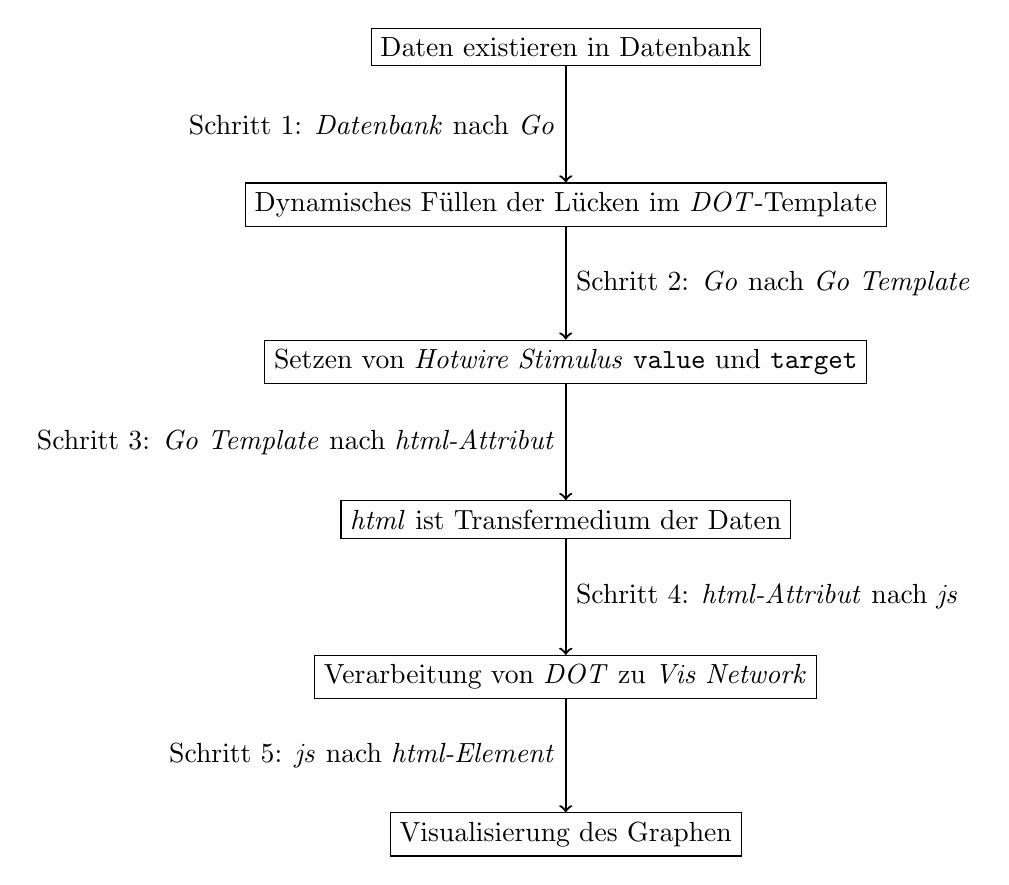
\begin{tikzpicture}[node distance=2cm, auto]

    % Nodes
    \node (start) [rectangle, draw, text centered] {Daten existieren in Datenbank};
    \node (process1) [rectangle, draw,below of=start] {Dynamisches Füllen der Lücken im \textit{DOT}-Template};
    \node (process2) [rectangle, draw,below of=process1] {Setzen von \textit{Hotwire Stimulus} \verb|value| und \verb|target|};
    \node (process3) [rectangle, draw,below of=process2] {\textit{\gls{html}} ist Transfermedium der Daten};
    \node (process4) [rectangle, draw,below of=process3] {Verarbeitung von \textit{DOT} zu \textit{Vis Network}};
    \node (stop) [rectangle, draw,below of=process4] {Visualisierung des Graphen};

    % Arrows
    \draw [->, thick] (start) -- (process1) node[midway, left] {Schritt 1: \textit{Datenbank} nach \textit{Go}};
    \draw [->, thick] (process1) -- (process2) node[midway, right] {Schritt 2: \textit{Go} nach \textit{Go Template}};
    \draw [->, thick] (process2) -- (process3) node[midway, left] {Schritt 3: \textit{Go Template} nach \textit{\gls{html}-Attribut}};
    \draw [->, thick] (process3) -- (process4) node[midway, right] {Schritt 4: \textit{\gls{html}-Attribut} nach \textit{\gls{js}}};
    \draw [->, thick] (process4) -- (stop) node[midway, left] {Schritt 5: \textit{\gls{js}} nach \textit{\gls{html}-Element}};

    \end{tikzpicture}
    \caption{Schritte zur Erstellung des Graphen}
    \label{fig:vis-graph-steps}
\end{figure}

\section{Sonstige Implementierungen}
Neben den bereits genannten Themen, wurden viele weitere kleinere Änderungen am Dashboard vorgenommen, um die Funktionalität und die Benutzererfahrung zu verbessern. Auf eine Auswahl dieser sonstigen Verbesserungen wird in diesem Kapitel eingegangen.
\subsection{Weiterführende Informationen zu Techniken}
\par Wie in Kapitel \ref{sec:datenquellen} beschrieben, bieten sich drei wissenschaftliche Konstruktur an, aus denen Techniken in die Matrix im Dashboard übernommen werden können. Bis auf zwei Techniken können alle im Dashboard angezeigten Techniken mindestens zwei Techniken aus \gls{tm4k}, \gls{mitre} \gls{attack} Matrix oder dem \gls{wg11} Report zugeordnet werden. Wie in \ref{sec:impl-anwendungVonAcema} beschrieben, wurde diese Zuweisung über einen Vergleich der Beschreibungen der jeweiligen Techniken manuell vorgenommen.
Um diese Zuweisungen nicht nur ohne weitere Funktion textuell darzustellen, wurde eine Verlinkung zu weiterführenden Informationen auf den Seiten \autocite{MITREATTCK} und \autocite{TacticsThreatMatrix} hinzugefügt. Eine Onlinequelle zu den O-RAN Bedrohungen gibt es bisher nicht, diese sind alleine in einem Microsoft Word Dokument veröffentlicht. Die URL, an die nach einem Klick weitergeleitet wird, ist dynamisch aus den Daten der Technik zusammengesetzt. Für die \gls{mitre} \gls{attack} Webseite setzt sich die URL so zusammen: \par \verb|attack.mitre.org/techniques/{Technik-ID}/{Subtechnik-ID}|
\par Microsofts \gls{tm4k} Seite nutzt für die URLs nicht die eindeutige ID, sondern den Titel der Technik. Die URL kann also wie folgt definiert werden: \par \verb|microsoft.github.io/Threat-Matrix-for-Kubernetes/techniques/{Technik-Titel}|
\par Die Zuordnung zu den Quellen wird auch farblich gekennzeichnet. Wenn kein Wert angezeigt wird, ist keine weitere Zuordnung möglich.
\subsection{Zoom- und Filterverhalten in der Zeitleiste}
\todo{Hier erklären, warum die Dumbbells angezeigt, nur max 100 Artefakte gleichzeitig angezeigt werden.
und verhalten der Start/Endzeit.}

\subsection{Vereinfachung der Datenstruktur eines Artefakts}
Über den Zeitraum der Implementierung haben sich nicht wenige Änderungen in der Datenstruktur eines Artefakts ergeben. In einer NoSQL Datenbank muss prinzipiell keine feste Struktur vorhanden sein muss, ist jedoch für das Auslesen eines Objekts in die definierte Datenstruktur in \textit{Go} nötig. Da die Serialisierung von Python zu JSON in einer anderen Anwendung und von anderen Personen implementiert wurde als die Deserialisierung von JSON zu Go, war eine Absprache von großer Wichtigkeit. So wurde aus dem Feld \verb|mitre| mit Datentyp \verb|String| zuerst eine Liste um auch eine Zuordnung zu mehreren \gls{mitre} Techniken abbilden zu können. Später wurden alle Informationen über Techniken und Taktik in ein Feld vereint. Das Feld \verb|command| wurde angepasst, um die Ausführung mehrerer Kommandos während eines Angriffs modellieren zu können. Weitere kleinere Änderungen führten zu dem Schema, welches im Anhang \ref{app:db-schema} dargestellt ist.